%auto-ignore
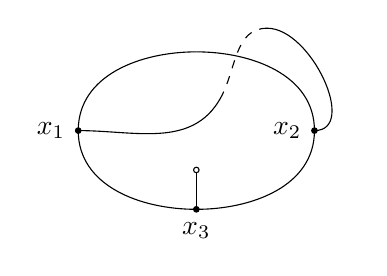
\begin{tikzpicture}
 \tikzset{point/.style = {draw, circle, fill=black, minimum size=2pt,inner sep=0pt}}
 \tikzset{->-/.style={decoration={markings,mark=at position #1 with {\arrow{>}}},postaction={decorate}}}
 
 \def\lenI{3cm}
 \def\lenII{1cm}
 \def\lenext{0.5cm}
 
 \coordinate (x1) at (0,0) {};
 \coordinate (x2) at (\lenI,0);
 \coordinate (x3) at (0.5*\lenI,-1*\lenII);

 \coordinate (p4) at (0.5*\lenI,\lenII);
 \coordinate (p5) at (0.6*\lenI,0.4*\lenII);
 \coordinate (p6) at (0.8*\lenI,1.3*\lenII);

 \draw (x1) to[out=90,in=180] (p4);
 \draw (p4) to[out=0,in=90] (x2);
 \draw (x1) to[out=-90,in=180] (x3);
 \draw (x3) to[out=0,in=-90] (x2);
 \draw (x1) to[out=0,in=-120] (p5);
 \draw[dashed] (p5) to[out=60,in=180] (p6);
 \draw (p6) to[out=0,in=0] (x2);
 
 \node[point,label={180:$x_1$}] at (x1) {};
 \node[point,label={180:$x_2$}] at (x2) {};
 \node[point,label={-90:$x_3$}] at (x3) {};
 
 \draw (x3) -- +(90:\lenext) node[point,,style={fill=white},label={180:$\NVol$}] {};
\end{tikzpicture}